\chapter*{Алгоритм генетического поиска для решения задачи планирования композитных приложений в распределенной вычислительной среде}
\addcontentsline{toc}{chapter}{2. Алгоритм генетического поиска для решения задачи планирования композитных приложений в распределенной вычислительной среде}
\begin{spacing}{1.3}

Генетический алгоритм поиска является универсальной концепцией для приближенного решения трудновычислимых задач. Его приложение к задаче планирования описано более подробно здесь \cite{GA}. Здесь же будет краткое описание работы алгоритма.

Общий вид генетического алгоритма одинаков для всех приложений:

\begin{algorithmic}
\STATE \textit{1. Инициализация начального поколения}
    \WHILE{Критерий остановки не выполнен}
    	\STATE \textit{2. Кроссовер} 
    	\STATE \textit{3. Мутация}
    	\STATE \textit{4. Оценка поколения}
    	\STATE \textit{5. Выбор в новое поколение хромосом}
    \ENDWHILE
\end{algorithmic}

Основную роль в генетическом алгоритме играет элемент поколения --- хромосома. В рамках задачи планирования хромосома выглядит как пара строк. Одна строка, будем называть её $mat$ задает соответствие между задачей и ресурсом. Вторая строка --- $ss$ задает последовательность задач в которой они будут запланированы. Важно что $ss$ является некоторой топологической сортировкой ацикличного графа композитного приложения.

В начальное поколение генетического алгоритма нужно добавлять совсем случайные хромосомы и хромосомы которые соответствуют решениям построенным другими различными эвристиками, например с помощью DLS или HEFT. Тогда генетический алгоритм может улучшить какое-то из решений с помощью случайных процессов которые происходят с хромосомами. 


Кроссовер является одной из наиболее важных частей алгоритма. Он помогает обмениваться информацией между двумя хромосомами --- создавать новые хромосомы отличные от родительских. Кроссовер между двумя $mat$ строками просто режет их в одинаковых частях и меняет отрезанные части. Кроссовер между двумя $ss$ строками также режет их в одинаковых местах и потом в отрезанной части строки задачи переставляются в порядке, задаваемым строкой с которой происходит кроссовер. 

Мутация позволяет создавать хромосомы с совсем новым решением. Процесс мутации для $mat$ строки очень простой --- выбирается случайная задача и ей в соответствие задается случайный ресурс. Мутация же $ss$ строки происходит чуть сложнее. Выбирается случайная задача и переносится в случайное место такое, чтобы новая строка также являлась топологической сортировкой.

Пример DAG и возможных строк $ss$ и $mat$ для данной DAG и вычислительной сети с тремя ресурсами.

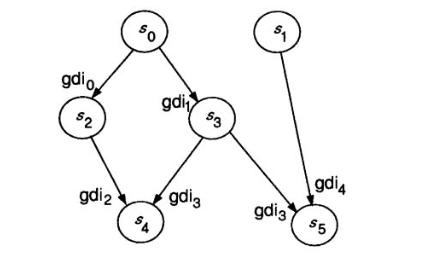
\includegraphics[width=85mm,height=60mm]{dag_example}
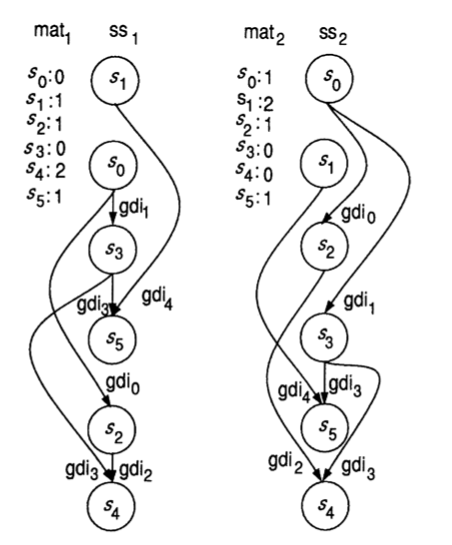
\includegraphics[width=75mm,height=80mm]{ss_mat_ex}

Оценка хромосомы осуществляется с помощью симуляции или того расписания которое было построено (оно дает приблизительное время выполнения композитного приложения так как в составлении расписания не учитывается общее пользование сети). После того как все элементы поколения получили оценку, они сортируются на основе этой оценки и потом в зависимости от места в порядке сортировки им присуждается вероятность с которой они будут выбраны. Выбор производится с повторением, то есть некоторые хромосомы могут дублироваться, однако это будут скорее всего хромосомы с хорошим расписанием. Для $i$-го элемента будет следующая вероятность: 
$$
P_i = R^{N - i - 1} (1 - R) / (1 - R^N)
$$
$N$ --- размер популяции, $R$ - параметр алгоритма.

Помимо $R$  у генетического алгоритма есть и другие параметры. Одни из них является размер популяции $N$. Также есть параметры связанные с мутацией и кроссовером. Процесс кроссовера происходит так --- популяция разбивается на $N/2$ пар и для каждой пары с вероятность $P_{crossover}$ происходит кроссовер. Аналогично существует и вероятность мутации $P_{mutation}$ для каждого элемента популяции. Кроме того, в данной адаптации есть параметр --- количество популяции, что есть просто количество итераций цикла. Удачная настройка этих параметров позволяет получать более качественные результаты. Однако, такую настройку можно произвести только сделав несколько  экспериментальных запусков алгоритма.




\end{spacing}